\graphicspath{{figures/AcceptanceTest/}}

\chapter{Inverted Pendulum Acceptance Tests}\label{sec:InvPendAccTest}

In this section the tests to check whether the controllers designed for the inverted pendulum fit the requirements or not. As said in \autoref{sec:TestDesc} the first acceptance test will not be documented as it is more an implementation requirement than a test.

\section{Acceptance Test 1.}

This test is there to verify the arm does indeed stop when it goes beyond $\frac{\pi}{4}$. To do so a large perturbation is applied to the stick such as the arm has to move beyond $\frac{\pi}{4}$ to catch it. It is confirmed then that the arm indeed stops at $\frac{\pi}{4}$.

So the test is considered as a success.

\section{Acceptance Test 2.}

The goal of this test is to see if the inverted pendulum's stick and arm stay within the limits set in Requirement 2 and 3 described in \autoref{sec:InvPendReq}. \autoref{fig:AccTest2Arm} and \ref{fig:AccTest2Stick} plot respectively the angles of the arm and the stick over a period of \SI{30}{\second}. The maximum and the minimum angles are put in evidence so that it is easy to compare them with the requirements.

\begin{figure} [htbp]
	\centering
	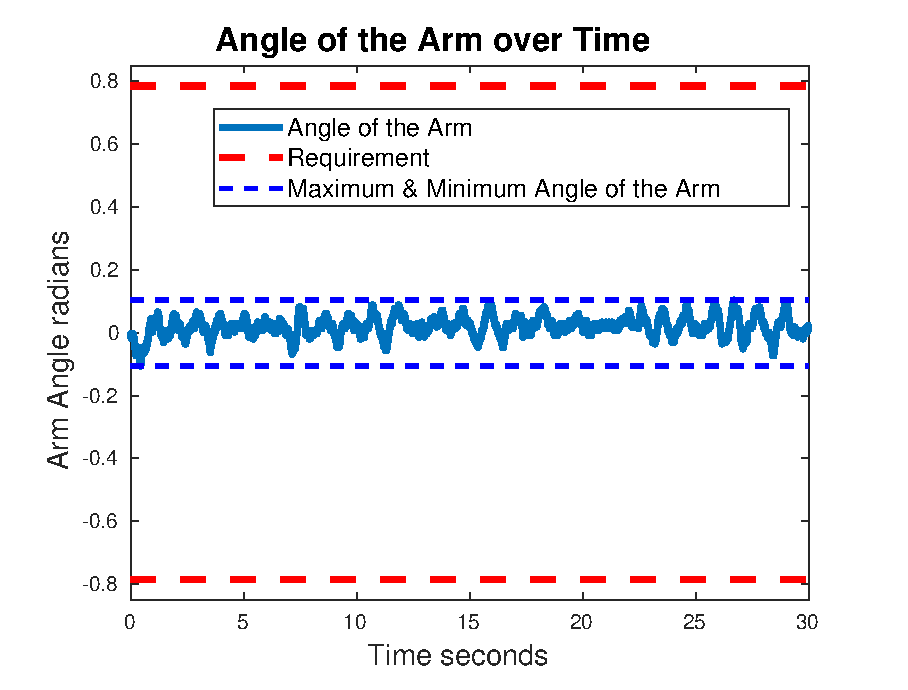
\includegraphics[width=0.6\textwidth]{AngleArmplot}
	\caption{Plot of the angle of the arm over time with the limits set by the Requirement 1.}
	\label{fig:AccTest2Arm}
\end{figure}

From \autoref{fig:AccTest2Arm} it can be seen that the arm is within the requirements by a large margin of \SI{0.68}{\radian} or \SI{38.96}{\degree}. This result is due to the transformation of the outer loop described in \autoref{subsec:InvPendOuterLoopRedef}. Indeed the reference is not the upright angle of the stick anymore but the distance of a point on the stick compared with its position when both the arm and the stick are in upright position. Due to this, the controller will try to keep both the arm and the stick in the upright angle which explains the very low angle variation of the arm compared to the requirement.

\begin{figure} [htbp]
	\centering
	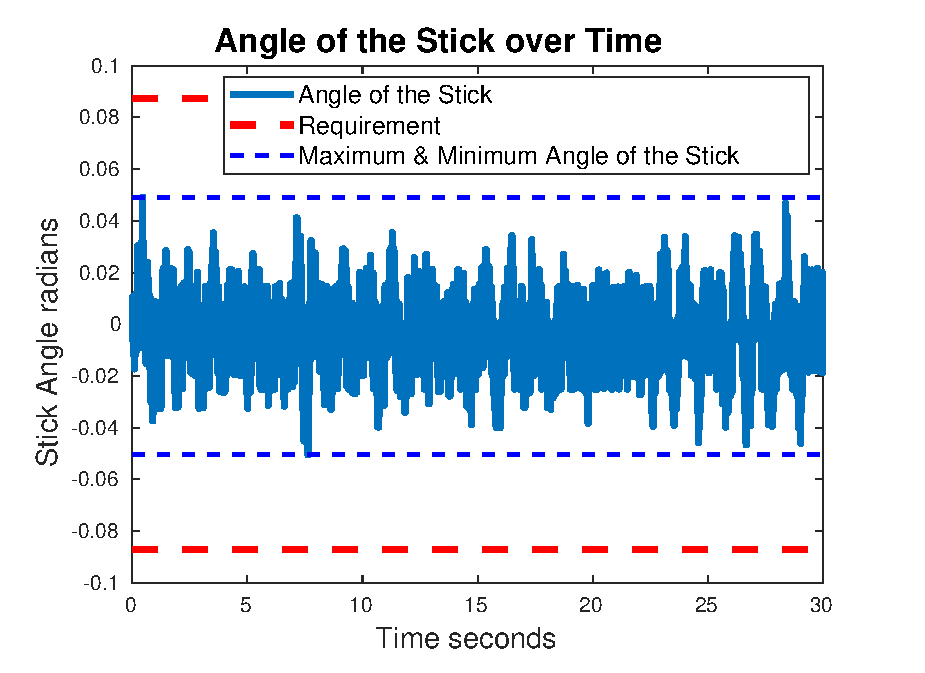
\includegraphics[width=0.6\textwidth]{AngleStickplot}
	\caption{Plot of the angle of the Stick over time with the limits set by the Requirement 2.}
	\label{fig:AccTest2Stick}
\end{figure}

In \autoref{fig:AccTest2Stick}, the largest angle the stick takes is \SI{0.05}{\radian} while Requirement 2 precises a limit of \SI{0.9}{\radian}. Again, the requirement is respected by a large margin.

From the tests results it can be concluded that the second acceptance test is a success.

\section{Acceptance Test 3.}

Unfortunately a method to precisely hold and release the stick was not found, therefore no precise data were able to be collected for this test. However, a video was taken during the test and will be joined with the report. This video in "AcceptanceTest/IPAcceptanceTest2" shows the reactions of the stick when different pushes are applied to it. The maximum angle for the stick set in the requirements are present and can be used as reference points. It can be noted that during the whole video the stick keeps its balance.

The results for the acceptance tests of the stick are a success.